\documentclass[11pt]{article}

% Change "review" to "final" to generate the final (sometimes called camera-ready) version.
% Change to "preprint" to generate a non-anonymous version with page numbers.
\usepackage[final]{acl}

% Standard package includes
\usepackage{latexsym}
\usepackage{booktabs}
\usepackage{amsmath}
\usepackage{amssymb}
\usepackage{stfloats}
\usepackage{tikz}
\usetikzlibrary{shapes.geometric,arrows.meta,positioning,fit,backgrounds}

% ---------------------------------------------------------------
% UNICODE FONTS -- requires the XeLaTeX compiler.
% fontenc/inputenc/CJKutf8 are pdfLaTeX-only and are replaced by
% fontspec. These define \mytext (Burmese), \jptext (Japanese),
% \zhtext (Chinese) and \fatext (Persian).
% ---------------------------------------------------------------
\usepackage{fontspec}
\newfontfamily\myanmarfont{Noto Sans Myanmar}
\newcommand{\mytext}[1]{{\myanmarfont #1}}
\newfontfamily\jptext{Noto Sans CJK JP}    % Japanese
\newfontfamily\zhtext{Noto Sans CJK SC}    % Chinese
\newfontfamily\fatext{Noto Naskh Arabic}   % Persian

% This is not strictly necessary, and may be commented out,
% but it will improve the layout of the manuscript,
% and will typically save some space.
\usepackage{microtype}


%Including images in your LaTeX document requires adding
%additional package(s)
\usepackage{graphicx}

% If the title and author information does not fit in the area allocated, uncomment the following
%
%\setlength\titlebox{<dim>}
%
% and set <dim> to something 5cm or larger.

\title{Improving Cross-lingual Word Representations for Burmese via Contextual Embedding Alignment and Transfer-Language Selection}

% Author information can be set in various styles:
% For several authors from the same institution:
% \author{Author 1 \and ... \and Author n \\
%         Address line \\ ... \\ Address line}
% if the names do not fit well on one line use
%         Author 1 \\ {\bf Author 2} \\ ... \\ {\bf Author n} \\
% For authors from different institutions:
% \author{Author 1 \\ Address line \\  ... \\ Address line
%         \And  ... \And
%         Author n \\ Address line \\ ... \\ Address line}
% To start a separate ``row'' of authors use \AND, as in
% \author{Author 1 \\ Address line \\  ... \\ Address line
%         \AND
%         Author 2 \\ Address line \\ ... \\ Address line \And
%         Author 3 \\ Address line \\ ... \\ Address line}

% Camera-ready: three authors, one shared affiliation to prevent overlap.
\author{Hsu Nyeint Thu \quad Aye Hninn Khine \quad Santitham Prom-on\\
King Mongkut's University of Technology Thonburi, Thailand\\
\texttt{hsunyeint.thu1@kmutt.ac.th}\\
\texttt{aye.hnin@kmutt.ac.th}\\
\texttt{santitham.pro@kmutt.ac.th}}

%\author{
%  \textbf{First Author\textsuperscript{1}},
%  \textbf{Second Author\textsuperscript{1,2}},
%  \textbf{Third T. Author\textsuperscript{1}},
%  \textbf{Fourth Author\textsuperscript{1}},
%\\
%  \textbf{Fifth Author\textsuperscript{1,2}},
%  \textbf{Sixth Author\textsuperscript{1}},
%  \textbf{Seventh Author\textsuperscript{1}},
%  \textbf{Eighth Author \textsuperscript{1,2,3,4}},
%\\
%  \textbf{Ninth Author\textsuperscript{1}},
%  \textbf{Tenth Author\textsuperscript{1}},
%  \textbf{Eleventh E. Author\textsuperscript{1,2,3,4,5}},
%  \textbf{Twelfth Author\textsuperscript{1}},
%\\
%  \textbf{Thirteenth Author\textsuperscript{3}},
%  \textbf{Fourteenth F. Author\textsuperscript{2,4}},
%  \textbf{Fifteenth Author\textsuperscript{1}},
%  \textbf{Sixteenth Author\textsuperscript{1}},
%\\
%  \textbf{Seventeenth S. Author\textsuperscript{4,5}},
%  \textbf{Eighteenth Author\textsuperscript{3,4}},
%  \textbf{Nineteenth N. Author\textsuperscript{2,5}},
%  \textbf{Twentieth Author\textsuperscript{1}}
%\\
%\\
%  \textsuperscript{1}Affiliation 1,
%  \textsuperscript{2}Affiliation 2,
%  \textsuperscript{3}Affiliation 3,
%  \textsuperscript{4}Affiliation 4,
%  \textsuperscript{5}Affiliation 5
%\\
%  \small{
%    \textbf{Correspondence:} \href{mailto:email@domain}{email@domain}
%  }
%}

\begin{document}
\maketitle
\begin{abstract}
Low-resource languages face significant challenges in natural language processing (NLP) due to limited annotated data, parallel corpora, and linguistic resources. Burmese remains underrepresented in multilingual NLP; although included in multilingual pre-trained models such as multilingual BERT (mBERT), its limited representation in pre-training data may constrain the quality of its cross-lingual representations. This paper investigates whether contextual cross-lingual embedding alignment can improve Burmese word retrieval without further pre-training or fine-tuning of the underlying encoder or parallel supervision.

We first rank candidate transfer languages for Burmese using LangRank, a LightGBM-based ranking model combining dataset, lexical, and linguistic similarity features, supplemented with typologically motivated choices. Contextual bilingual word pairs are then mined automatically from monolingual corpora through nearest-neighbour search over frozen encoder representations. A lightweight linear transformation is trained on these pairs to align Burmese representations with each transfer language while leaving the encoder unchanged.

We evaluate cross-lingual word retrieval across five Burmese–X pairs: Vietnamese, Persian, Turkish, Japanese, and Chinese, using mBERT and LaBSE as frozen backbones. With mBERT, alignment improves retrieval accuracy over the frozen baseline for all five pairs, with relative gains of 16\%–124\%. Multi-seed experiments confirm statistically significant improvements ($p<0.05$) across all pairs. In contrast, alignment degrades LaBSE retrieval across all five pairs and three examined seeds per pair, while frozen LaBSE achieves the strongest overall performance. These contrasting results show that the effectiveness of contextual alignment is backbone-dependent: it can substantially improve weaker multilingual representations such as mBERT, but may disrupt already well-aligned representations such as LaBSE.
\end{abstract}

\section{Introduction}

Recent advances in multilingual pre-trained language models (PLMs), such as
multilingual BERT (mBERT) \citep{devlin-etal-2019-bert}, have substantially
improved cross-lingual transfer. However, performance remains uneven across
languages, particularly for those with limited representation in pre-training data. For Burmese, improving cross-lingual
representations through supervised approaches is additionally constrained by
the scarcity of large parallel corpora and bilingual lexicons.

One approach to addressing this limitation is contextual cross-lingual embedding alignment, which improves multilingual representations without retraining the underlying model. The Contextualized Cross-lingual Word Representation (CCWR) \citep{hangya-etal-2022-improving} framework aligns contextual embeddings using automatically mined bilingual word pairs while keeping the encoder frozen, requiring neither full-model fine-tuning nor large parallel corpora -- but its effectiveness may vary with the choice of transfer language, and its behaviour on Burmese has not been systematically studied. Selecting transfer languages well is itself an open question: transfer performance varies with linguistic similarity, lexical overlap, and data availability, and tools such as LangRank \citep{lin-etal-2019-choosing} offer a systematic way to shortlist candidates, but there is little empirical evidence on which languages actually help Burmese once contextual alignment is applied.

We use LangRank to rank candidate transfer languages for Burmese, supplemented with two additional languages (Chinese, Japanese) chosen for typological proximity, then mine contextual bilingual word pairs from monolingual corpora using a frozen encoder and train a lightweight linear alignment layer on them, following CCWR. We evaluate the aligned representations through cross-lingual word retrieval
across five Burmese--X language pairs: Vietnamese, Persian, Turkish, Japanese,
and Chinese. The experiments examine whether contextual embedding alignment
improves retrieval over the original frozen representations, how performance
varies with the choice of transfer language and the amount of monolingual
training data, and whether the effect of alignment differs between mBERT and
LaBSE.
The main contributions of this paper are threefold. First, we present a systematic empirical study of contextual cross-lingual embedding alignment for Burmese, a low-resource language that has received limited attention in multilingual representation learning. Second, we evaluate LangRank-based transfer-language selection for Burmese and combine it with typologically motivated additions, comparing five candidate transfer languages with different linguistic characteristics. Third, we examine how transfer-language choice, monolingual corpus size, and encoder backbone
affect the effectiveness of contextual embedding alignment.

\section{Related Work}

\subsection{Cross-lingual Embedding Alignment} 
Aligning word or contextual embeddings across languages into a shared space to support cross-lingual transfer originates with linear mappings between static embedding spaces learned from a bilingual dictionary \citep{mikolov-etal-2013-exploiting}; later work removed the need for a seed dictionary via adversarial training \citep{lample-etal-2018-word} or iterative self-learning \citep{artetxe-etal-2018-robust}. More recent work extends this to contextual representations from pre-trained multilingual encoders \citep{schuster-etal-2019-cross}. The CCWR framework we build on \citep{hangya-etal-2022-improving} targets low-resource languages specifically: it keeps the encoder frozen and learns only lightweight linear transformations on automatically mined, rather than dictionary-based, word pairs. Our mining step (Section~\ref{sec:mining}) also draws on SimAlign \citep{jalili-sabet-etal-2020-simalign}, which we use to generate word alignments for all five pairs in Section~\ref{sec:data_prep}; the same conversion pipeline is applied to the OpenSubtitles-derived Burmese--Turkish and Burmese--Persian pairs, for which the ALT-specific sentence-ID stripping step is a no-op.

\subsection{Transfer Language Ranking} 
LangRank \citep{lin-etal-2019-choosing}, used in Stage~1 of this study, formulates transfer-language selection as learning-to-rank over dataset, lexical, and linguistic-distance features. A complementary line of work studies \emph{why} multilingual models such as mBERT transfer across languages at all, finding transfer strongest between typologically similar languages \citep{pires-etal-2019-multilingual,karthikeyan-etal-2020-cross}, which motivates our use of typological evidence to add Chinese and Japanese as transfer languages (Section~\ref{sec:transfer_selection}) beyond LangRank's own output. \citet{ruder-etal-2019-survey} survey this broader space; Burmese has not been a particular focus of it.

\subsection{Burmese NLP} 
NLP resources for Burmese remain scarce, with existing work concentrated on word/syllable segmentation \citep{ding-etal-2016-word} and corpus construction, notably the Asian Language Treebank \citep{thu-etal-2016-introducing}, which we also use for evaluation (Section~\ref{sec:datasets}). \citet{mao-etal-2022-burmese} adapt an English-pretrained sentiment classifier to Burmese via full task fine-tuning, rather than representation alignment. General-purpose multilingual encoders continue to scale \citep{devlin-etal-2019-bert,conneau-etal-2020-unsupervised,artetxe-schwenk-2019-massively}, but their cross-lingual transfer quality remains highly uneven across languages, correlating with pre-training data volume \citep{wu-dredze-2019-beto,wu-dredze-2020-languages} -- precisely the gap this paper investigates for Burmese, where cross-lingual \emph{representation alignment} specifically, as opposed to segmentation, corpus construction, or task fine-tuning, has received little attention.

\section{Methodology}

\subsection{Framework Overview}

This study investigates multilingual contextual embedding alignment for improving cross-lingual word representations of Burmese, a low-resource language. Rather than fine-tuning or continuing to pre-train the underlying multilingual encoder, the selected framework keeps the encoder frozen throughout and instead learns a lightweight, per-language-pair transformation on top of it. The framework consists of two stages. Stage 1 selects transfer languages for Burmese using LangRank. Stage 2, built around the CCWR (Contextualized Cross-lingual Word Representation) procedure, covers everything from monolingual and parallel corpus preparation, through contextual bilingual word-pair mining, to embedding alignment and word-retrieval evaluation. Figure~\ref{fig:architecture} illustrates how these two stages connect; Section~\ref{sec:transfer_selection} details Stage 1 and Sections~\ref{sec:data_prep}--\ref{sec:alignment} detail Stage 2.

\begin{figure*}[t]
\centering
\resizebox{\textwidth}{!}{%
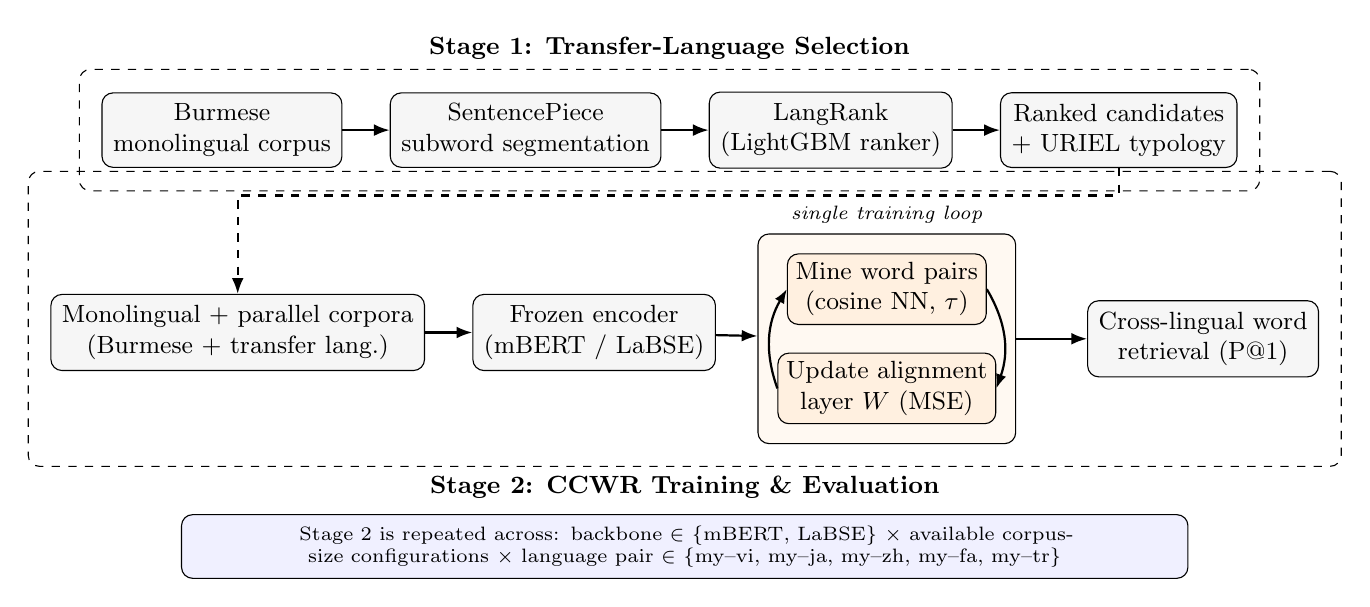
\begin{tikzpicture}[
  font=\small,
  box/.style={draw, rounded corners, align=center, minimum height=0.9cm, inner sep=4pt, fill=gray!7},
  innerbox/.style={draw, rounded corners, align=center, minimum height=0.8cm, inner sep=3pt, fill=orange!12},
  stage/.style={draw, dashed, rounded corners, inner sep=8pt},
  loopbox/.style={draw, rounded corners, inner sep=6pt, fill=orange!5},
  arrow/.style={-{Latex[length=2mm]}, thick},
  looparrow/.style={-{Latex[length=1.8mm]}, thick, bend left=25}
]

% ---- Stage 1: transfer language selection ----
\node[box, minimum width=2.6cm] (mono) {Burmese\\monolingual corpus};
\node[box, right=0.6cm of mono, minimum width=2.6cm] (spm) {SentencePiece\\subword segmentation};
\node[box, right=0.6cm of spm, minimum width=2.6cm] (langrank) {LangRank\\(LightGBM ranker)};
\node[box, right=0.6cm of langrank, minimum width=3.0cm] (ranked) {Ranked candidates\\+ URIEL typology};

\draw[arrow] (mono) -- (spm);
\draw[arrow] (spm) -- (langrank);
\draw[arrow] (langrank) -- (ranked);

\node[stage, fit=(mono)(spm)(langrank)(ranked), label={[font=\small\bfseries]above:Stage 1: Transfer-Language Selection}] (stage1) {};

% ---- Stage 2: CCWR training ----
\node[box, below=1.6cm of mono, xshift=0.2cm, minimum width=2.6cm] (mono2) {Monolingual + parallel corpora\\(Burmese + transfer lang.)};
\node[box, right=0.6cm of mono2, minimum width=2.4cm] (mbert) {Frozen encoder\\(mBERT / LaBSE)};

\node[innerbox, right=0.9cm of mbert, minimum width=2.3cm, yshift=0.55cm] (mine) {Mine word pairs\\(cosine NN, $\tau$)};
\node[innerbox, below=0.35cm of mine, minimum width=2.3cm] (train) {Update alignment\\layer $W$ (MSE)};
\begin{pgfonlayer}{background}
\node[loopbox, fit=(mine)(train), inner sep=7pt, label={[font=\scriptsize\itshape, text=black, fill=none]above:single training loop}] (loop) {};
\end{pgfonlayer}
\node[inner sep=0pt, minimum height=0pt] (spacer) at ([yshift=0.5cm]loop.north) {};

\node[box, right=0.9cm of loop, minimum width=2.4cm] (eval) {Cross-lingual word\\retrieval (P@1)};

\draw[arrow] (mono2) -- (mbert);
\draw[arrow] (mbert) -- (loop);
\draw[looparrow] (mine.east) to (train.east);
\draw[looparrow] (train.west) to (mine.west);
\draw[arrow] (loop) -- (eval);

\node[stage, fit=(mono2)(mbert)(loop)(eval)(spacer), label={[font=\small\bfseries]below:Stage 2: CCWR Training \& Evaluation }] (stage2) {};

\draw[arrow, dashed] (ranked.south) -- ++(0,-0.35) -| (mono2.north);

\node[box, below=0.6cm of stage2.south, text width=12.5cm, align=center, minimum height=0.7cm, fill=blue!6, font=\scriptsize] (sweep)
  {Stage 2 is repeated across:
backbone $\in$ \{mBERT, LaBSE\}
$\times$ available corpus-size configurations
$\times$ language pair $\in$ \{my--vi, my--ja, my--zh, my--fa, my--tr\}};


\end{tikzpicture}%
}
\caption{Overview of the experimental framework (Stage 1 selects transfer languages for Burmese using LangRank features together with typological evidence from URIEL. Stage 2 prepares corpora, then runs a single training loop in which word-pair mining and linear alignment-layer training are interleaved at every step, not run as separate preprocessing and training stages, before evaluating via cross-lingual word retrieval. As summarized at the bottom, Stage 2 is run across the available combinations of backbone (mBERT or LaBSE), monolingual corpus size (20k or 40k sentences), and Burmese--transfer-language pair, giving the full set of results reported in Section~\ref{sec:results}.}
\label{fig:architecture}
\end{figure*}

\subsection{Transfer Language Selection}
\label{sec:transfer_selection}

Rather than choosing transfer languages by intuition, we first rank candidate languages using LangRank \citep{lin-etal-2019-choosing}, which predicts the usefulness of a source language for cross-lingual transfer from dataset, lexical, and linguistic-distance features (drawn from URIEL, a multilingual
typological database). Two SentencePiece models were trained on Burmese text at different scales, a small BPE model on a 20{,}106-sentence corpus and a larger model on a cleaned Wikipedia dump of 774{,}506 sentences, and LangRank was run against each. The smaller corpus ranked Persian, Turkish, and Hungarian above Vietnamese; the larger, cleaner corpus shifted the ranking, promoting Vietnamese to first place, indicating LangRank's dataset features are themselves sensitive to corpus size and cleaning quality for an under-resourced language like Burmese. Discarding a self-match artefact, the two runs together support Vietnamese, Persian, and Turkish as the empirically preferred transfer languages, with Bulgarian appearing in the ranking but not carried forward, as it is typologically distant (Slavic, Indo-European) from Sino-Tibetan Burmese.

Because LangRank's dataset-driven features favour large, easily obtained corpora and can underweight typological fit, we complement the ranking with two additional languages, Chinese and Japanese, chosen on typological and regional grounds. In the URIEL single-feature rankings, Chinese
appears among the closest candidates under genetic distance, while Japanese
appears among the closest under syntactic and featural distance. The final set of five transfer languages is therefore Vietnamese, Persian, Turkish, Japanese, and Chinese. Full LangRank scores and selection rationale are in Appendix~\ref{app:method_details}.

\subsection{Multilingual Data Preparation}
\label{sec:data_prep}

Monolingual corpora for Burmese and each transfer language are collected from Wikipedia and cleaned with language-specific filters. Twenty thousand cleaned sentences per language are sampled for the main experiments (Appendix~\ref{app:corpus_stats}); a larger, 40,000-sentence configuration is additionally prepared to examine corpus-size effects (Appendix~\ref{app:ablations}), although Japanese and Chinese do not reach the 40k target. Full corpus statistics are provided in Appendix~\ref{app:corpus_stats}. Parallel data is used only for evaluation: Burmese--Vietnamese, Burmese--Japanese, and Burmese--Chinese pairs are from the Asian Language Treebank \citep[ALT;][]{thu-etal-2016-introducing}; Burmese--Turkish and Burmese--Persian, for which ALT has no coverage, are taken from the direct bitexts released in OPUS OpenSubtitles v2024 \citep{lison-tiedemann-2016-opensubtitles}. All evaluation datasets are subsampled to 20,106 sentence pairs to control evaluation-set size, not retrieval-candidate-pool size. Paired sentences are stored as whitespace-tokenized \texttt{.tokens} files, and SimAlign \citep{jalili-sabet-etal-2020-simalign} with BPE and IterMax produces automatic word-index references in \texttt{.alignments} files. The evaluation loader retains one-to-one alignments. These are silver references, not manually verified translations. The parallel data and their references are used for validation and testing, not to supervise the alignment layer, which trains on pairs mined from separate monolingual Wikipedia corpora.

\subsection{Contextual Bilingual Word-Pair Mining}
\label{sec:mining}

Given monolingual corpora in Burmese and a transfer language, contextual word representations are extracted using the pretrained, frozen encoder; its parameters are never updated. Following CCWR, bilingual word pairs are mined automatically by treating each Burmese contextual embedding as a query and retrieving its nearest neighbour in the transfer language's embedding space via cosine similarity:

\begin{equation}
\mathrm{sim}(\mathbf{x}, \mathbf{y}) = \frac{\mathbf{x}^{\top}\mathbf{y}}{\lVert \mathbf{x}\rVert \, \lVert \mathbf{y}\rVert},
\label{eq:cosine}
\end{equation}

retaining a pair $(\mathbf{x}, \mathbf{y})$ only if similarity exceeds a fixed threshold $\tau = 0.2$ (and falls below an upper bound of 100, which excludes near-duplicate pairs). This is not a one-off preprocessing pass: mining and alignment-layer training are interleaved within a single loop, with fresh batches re-mined at regular intervals using the alignment layer's current state. This requires no bilingual dictionary and no parallel corpus, making the approach applicable where both are scarce.

\subsection{Cross-lingual Embedding Alignment}
\label{sec:alignment}

The central component is a lightweight alignment step improving cross-lingual consistency between Burmese and each transfer language without touching the encoder itself. Let $\mathbf{x} \in \mathbb{R}^{d}$ denote the frozen representation of a Burmese word and $\mathbf{y} \in \mathbb{R}^{d}$ its mined counterpart. We learn a linear transformation matrix $\mathbf{W} \in \mathbb{R}^{d \times d}$, specific to each pair, such that

\begin{equation}
\mathbf{W}\mathbf{x} \approx \mathbf{y},
\label{eq:map}
\end{equation}

optimized by minimizing mean squared error over all mined pairs $(\mathbf{x}_i, \mathbf{y}_i)$:

\begin{equation}
\mathcal{L}(\mathbf{W}) = \sum_{i} \left\lVert \mathbf{W}\mathbf{x}_i - \mathbf{y}_i \right\rVert_2^{2}.
\label{eq:loss}
\end{equation}

Only $\mathbf{W}$ is updated; the encoder parameters remain fixed throughout. At inference, a Burmese query is passed through the trained $\mathbf{W}$ before comparison against transfer-language representations, so retrieval takes place in a space where the two languages have been explicitly pulled together.

\section{Experimental Setup}
\label{sec:exp_setup}

\subsection{Training Setup}
\label{sec:datasets}

Table~\ref{tab:parallel_dataset} summarizes the parallel corpora used exclusively for evaluation. All five datasets contain 20,106 sentence pairs for consistency
across language pairs.

\begin{table}[h]
\centering
\small
\setlength{\tabcolsep}{4pt}
\caption{Parallel corpora used for evaluation only. All five were subsampled to the same size (20,106 sentence pairs) for consistency across language pairs.}
\label{tab:parallel_dataset}
\begin{tabular}{llr}
\toprule
\textbf{Pair} & \textbf{Source} & \textbf{\# Sent.} \\
\midrule
Burmese--Vietnamese & ALT           & 20,106 \\
Burmese--Japanese & ALT           & 20,106 \\
Burmese--Chinese & ALT           & 20,106 \\
Burmese--Turkish & OPUS OpenSubtitles & 20,106 \\
Burmese--Persian & OPUS OpenSubtitles & 20,106 \\
\bottomrule
\end{tabular}
\end{table}

The alignment layer was trained independently for each language pair using AdamW with a learning rate of $5\times10^{-5}$, batch size 2, gradient accumulation of 6, and up to 5,000 steps. Runs used approximately 18,053--18,058 training samples, with 1,024 examples each for validation and testing. All three runs used the same input data paths and experimental configuration, with the random seed varied to assess run-to-run variability. The forward-versus-intersection alignment ablation is reported in Appendix~\ref{app:ablations}.

\subsection{Baseline Models}
\label{sec:baselines}

The multilingual encoder is \texttt{bert-base-multilingual-cased}, used only in inference mode; its weights are never updated. Since the goal is to isolate the effect of alignment itself, we compare against a direct, frozen baseline: the encoder used for retrieval \emph{without} an alignment layer ($\mathbf{W} = \mathbf{I}$), evaluated on the same test splits, so any accuracy difference is attributable to the learned alignment.

To examine whether the effect of CCWR depends on the underlying
pretrained encoder, we repeat the 20k configurations with
\texttt{sentence-transformers/LaBSE} \citep{feng-etal-2022-language}
as an alternative frozen backbone for all five pairs, and the available
40k configurations for the three pairs that reach the 40k target,
keeping every other hyperparameter identical. LaBSE shares mBERT's BERT-style Transformer architecture but is pretrained with a multilingual bitext-retrieval objective across 109 languages rather than monolingual masked-language-modelling objective. Both frozen and CCWR-aligned LaBSE are reported alongside mBERT in Section~\ref{sec:backbone_comparison}.

\subsection{Retrieval Evaluation}
\label{sec:eval_metrics}

Alignment quality is measured through bilingual word retrieval. For each source-language representation, target-language candidates are ranked using Cross-domain Similarity Local Scaling (CSLS) \citep, whereas cosine similarity is used for training-pair mining. A retrieval is counted as correct when the top-ranked candidate matches the silver-standard token alignment automatically generated by SimAlign. We report Precision@1 (P@1),

\begin{equation}
P@1 = \frac{N_{\mathrm{correct}}}{N_{\mathrm{total}}} \times 100,
\label{eq:p1}
\end{equation}

separately for a \emph{contextual} setting, in which token representations are evaluated in their original sentence contexts, and a \emph{non-contextual} setting, in which unique token forms are used to construct a deduplicated retrieval candidate pool. The evaluation units follow the whitespace segmentation and subword handling of the prepared input, so a candidate need not correspond to the same linguistic unit across scripts. An overall score is computed as the mean of contextual and non-contextual accuracies for each pair, with results averaged over src$\to$trg and trg$\to$src retrieval directions.

\section{Results and Discussion}
\label{sec:results}

\subsection{Alignment Effectiveness}
\label{sec:overall_performance}

Table~\ref{tab:main_results} reports retrieval accuracy for the frozen mBERT baseline and for the experimental CCWR-aligned model, on the 20k-sentence, forward-alignment configuration, across all five Burmese--transfer-language pairs, broken down by contextual, non-contextual, and overall (averaged) accuracy. Contextual embedding alignment improves overall retrieval accuracy for
every pair, showing that a lightweight linear transformation can recover
additional cross-lingual signal from the frozen mBERT representations
without further pre-training. Improvement is driven mainly by the non-contextual (type-level) metric for every pair except Burmese--Vietnamese, whose overall gain comes primarily from contextual retrieval instead.

\begin{table}[t]
\centering
\small
\caption{Retrieval accuracy (P@1) by metric, frozen mBERT vs.\ + mBERT aligned with CCWR (20k, forward-alignment).}
\label{tab:main_results}
\setlength{\tabcolsep}{4pt}
\begin{tabular}{lcc|cc|cc|r}
\toprule
& \multicolumn{2}{c|}{\textbf{Context}} & \multicolumn{2}{c|}{\textbf{Non-ctx.}} & \multicolumn{2}{c|}{\textbf{Overall}} & \\
\textbf{Pair} & Fr. & +C & Fr. & +C & Fr. & +C & $|C|$ \\
\midrule
my--zh & 2.31 & 4.07 & 8.50 & 15.03 & 5.40 & 9.55 & 153 \\
my--ja & 2.32 & 4.24 & 8.94 & 11.59 & 5.63 & 7.92 & 151$^{\dagger}$ \\
my--vi & 2.41 & \textbf{5.98} & 4.00 & 8.43  & 3.21 & 7.20 & 2{,}925 \\
my--fa & 1.24 & 1.67 & 5.19 & 6.43  & 3.22 & 4.05 & 568$^{\dagger}$ \\
my--tr & 1.13 & 1.30 & 4.01 & 4.63  & 2.57 & 2.97 & 561$^{\dagger}$ \\
\midrule
\textbf{Avg.} & \textbf{1.88} & \textbf{3.45} & \textbf{6.13} & \textbf{9.22} & \textbf{4.01} & \textbf{6.34} & \\
\bottomrule
\end{tabular}
\\[2pt]
\raggedright\footnotesize ``Fr.'' = frozen mBERT; ``+C'' = mBERT with CCWR. $|C|$ is the number of candidates in the non-contextual retrieval pool, which differs by up to 19$\times$ across pairs and is therefore reported alongside the raw accuracies. $^{\dagger}$Derived from the retrieval-accuracy denominators; this reproduces the directly instrumented values for my--vi and my--zh exactly.
\end{table}

\subsection{Transfer-Language Effects}
\label{sec:transfer_analysis}

Table~\ref{tab:main_results} compares the effect of transfer-language choice. Based on the raw overall accuracy, Chinese ranks highest (9.55), followed by Japanese (7.92) and Vietnamese (7.20). However, these percentages are not directly comparable because the non-contextual retrieval candidate pools differ substantially in size. As discussed in Section~\ref{sec:error_analysis}, mBERT represents Chinese and Japanese largely as individual characters, resulting in candidate pools of approximately 150 items, whereas Burmese--Vietnamese contains 2,925 unique items. Thus, retrieval from the Chinese and Japanese pools is considerably easier. This is also reflected in the absolute numbers: Burmese--Chinese retrieves 25 and 21 items correctly in the two directions, compared with 255 and 238 for Burmese--Vietnamese.

For the non-contextual metric, normalizing accuracy by the corresponding chance level ($100/|C|$) changes the ranking. Burmese--Vietnamese achieves approximately 246 times chance, followed by Persian (37), Turkish (26), Chinese (23), and Japanese (18). Vietnamese also achieves the highest contextual retrieval accuracy (5.98\%), which is less affected by differences in candidate-pool size. Furthermore, alignment produces larger improvements for Vietnamese, with gains of $\times2.48$ for contextual retrieval and $\times2.11$ for non-contextual retrieval, compared with $\times1.76$ and $\times1.77$ for Chinese. The contextual ranking is also consistent across the three random seeds reported in Appendix~\ref{app:significance}.

Under the present evaluation configuration, Vietnamese achieves the strongest contextual accuracy and chance-normalized non-contextual retrieval performance, whereas Chinese obtains the highest raw overall P@1. This pattern is consistent with Vietnamese's top LangRank ranking (Section~\ref{sec:transfer_selection}), although the observed differences may also reflect variation in candidate-pool size, tokenization, and evaluation domains. Word-order similarity alone does not explain the results, as Japanese, Turkish, and Persian are also predominantly verb-final but achieve lower performance.

\subsection{Corpus-Size Effects}
\label{sec:corpus_size}

We next examine whether increasing the amount of monolingual data improves alignment performance. Table~\ref{tab:corpus_size_combined} compares the 20k and 40k configurations
for the three language pairs that reached the 40k target.

\begin{table}[h]
\centering
\small
\setlength{\tabcolsep}{4pt}
\caption{Effect of scaling the monolingual corpus from 20k to 40k on overall P@1, both backbones. Only pairs reaching the 40k target are shown.}
\label{tab:corpus_size_combined}
\begin{tabular}{lrr}
\toprule
\textbf{Pair} & \textbf{mBERT $\Delta$} & \textbf{LaBSE $\Delta$} \\
\midrule
my--vi & +0.05 & +0.00 \\
my--tr & -- & $-$0.29 \\
my--fa & -- & $-$0.22 \\
\bottomrule
\end{tabular}
\end{table}

Across the available 40k configurations, scaling the corpus changes overall accuracy by at most 0.29 points in either direction, suggesting limited benefit from
additional monolingual data at this scale.

\subsection{Backbone Effects}
\label{sec:backbone_comparison}

To test whether the gains reported above are specific to mBERT or reflect a more general property of the CCWR alignment procedure, we repeat the full experiment with LaBSE substituted as the frozen backbone, for all five Burmese--transfer-language pairs, at the 20k configuration. Critically, we evaluate LaBSE both \emph{with} CCWR alignment, mirroring the mBERT setup, and \emph{without} it, i.e.\ the frozen LaBSE encoder used for retrieval directly with $\mathbf{W} = \mathbf{I}$, exactly as the frozen-mBERT baseline in Section~\ref{sec:baselines} is evaluated. This second condition is what makes it possible to separate a genuine effect of the alignment procedure from a difference in what the two encoders already knew before any CCWR training began. Table~\ref{tab:labse_comparison} reports all four resulting configurations.

\begin{table}[h]
\centering
\small
\caption{Overall P@1 for both backbones, frozen and CCWR-aligned, in the original 20k seed-42 runs. $\Delta$ is the absolute percentage-point change. LaBSE three-seed results appear in Appendix~\ref{app:labse_seeds}.}
\label{tab:labse_comparison}
\begin{tabular}{lccc}
\toprule
\textbf{Pair} & \textbf{Frozen} & \textbf{+CCWR} & \textbf{$\Delta$} \\
\midrule
\multicolumn{4}{l}{\emph{mBERT}} \\
my--vi & 3.21  & 7.20  & +3.99 \\
my--ja & 5.63  & 7.92  & +2.29 \\
my--zh & 5.40  & 9.55  & +4.15 \\
my--fa & 3.22  & 4.05  & +0.83 \\
my--tr & 2.57  & 2.97  & +0.40 \\
\midrule
\multicolumn{4}{l}{\emph{LaBSE}} \\
my--vi & 46.23 & 44.26 & $-$1.97 \\
my--ja & 71.74 & 68.38 & $-$3.36 \\
my--zh & 71.93 & 65.43 & $-$6.50 \\
my--fa & 36.15 & 28.39 & $-$7.76 \\
my--tr & 39.50 & 30.17 & $-$9.33 \\
\bottomrule
\end{tabular}
\end{table}

The result is consistent across all five evaluated language pairs: CCWR alignment improves overall retrieval accuracy for every one of the five pairs under mBERT, and \emph{degrades} it for every one of the five pairs under LaBSE. The direction flips completely with the backbone, and the magnitude for mBERT (+0.40 to +4.15 points) is consistently far smaller than for LaBSE ($-$1.97 to $-$9.33 points). Frozen LaBSE alone, with no alignment training, is the best-performing configuration in this study for every pair -- a gap that is present, and larger, before any alignment happens, and that alignment training subsequently narrows by pulling LaBSE's representations \emph{away} from their pre-trained state. The pattern of performance changes across language pairs suggests that the quality of the mined supervision may be an important factor in determining the effect of alignment. If alignment harmed LaBSE primarily because its original representations were already strong, pairs with higher frozen accuracy would be expected to experience larger degradation. Instead, Burmese--Persian and Burmese--Turkish have the lowest frozen LaBSE accuracies (36.15 and 39.50) but show the largest relative decreases after alignment ($-21.5\%$ and $-23.6\%$), whereas Burmese--Vietnamese and Burmese--Japanese show much smaller decreases ($-4.3\%$ and $-4.7\%$). The pattern is also associated with the data source: the three ALT-derived pairs decrease by an average of 6.0\%, compared with 22.5\% for the two OpenSubtitles-derived pairs. A similar pattern is observed for mBERT, which gains 41--124\% on the ALT pairs but only 16--26\% on the OpenSubtitles pairs. This pattern is consistent with the hypothesis that the ALT-derived data produces cleaner mined supervision than the OpenSubtitles-derived data. This interpretation is consistent with the CCWR training procedure. The alignment layer minimizes mean squared error using automatically mined word pairs selected at a similarity threshold of $\tau=0.2$, without a curated dictionary or negative sampling. Consequently, noisy pairs can directly pull representations toward incorrect counterparts. For mBERT, whose cross-lingual representations are relatively weak, even imperfect supervision may provide a net benefit. In contrast, LaBSE starts with stronger lexical representations, making it more sensitive to noisy alignment targets. This interpretation is also consistent with \citet{vulic-etal-2023-probing}, who improved LaBSE word-level retrieval by 9.4 P@1 using a contrastive objective trained on gold translation pairs. Thus, our results suggest that LaBSE can benefit from lexical alignment when cleaner supervision is available, and that the degradation observed here is more likely a limitation of the automatically mined supervision than of LaBSE itself. However, given the small number of language pairs and the confounding between data source and language pair, this explanation should be regarded as a plausible interpretation rather than a demonstrated causal effect. These results suggest that CCWR may be unnecessary or detrimental for
a backbone whose pre-training already explicitly targets cross-lingual
alignment, whereas it remains beneficial for mBERT under the evaluated
setting.

\subsection{Diagnostic \& Robustness Analyses}
\label{sec:error_analysis}

To ground the aggregate accuracy numbers reported above in concrete model behaviour, we extract per-item, non-contextual retrieval predictions for all five pairs under mBERT+CCWR at the 20k configuration and inspect them directly. This analysis covers the mBERT backbone only.

Table~\ref{tab:cross_pair_errors} summarizes three statistics per pair: the share of queries retrieved correctly, the share of those correct retrievals that are trivial numeral-to-numeral matches (e.g.\ a digit string retrieving the same digit string, reflecting literal identity rather than learned correspondence), and hub attraction, the share of all errors accounted for by the 15 most frequently mispredicted words.

\begin{table}[h]
\centering
\small
\caption{Error statistics from per-item, non-contextual retrieval predictions (mBERT+CCWR, 20k configuration).}
\label{tab:cross_pair_errors}
\begin{tabular}{lcccc}
\toprule
\textbf{Pair} & \textbf{\# Queries} & \textbf{Correct} & \textbf{Numeral} & \textbf{Hub} \\
\midrule
my--vi & 11,704 & 8.2\%  & 11.3\% & 10.5\% \\
my--ja & 531    & 12.8\% & 2.9\%  & 57.9\% \\
my--zh & 568    & 14.8\% & 2.4\%  & 47.9\% \\
my--fa & 1,802  & 5.7\%  & 14.6\% & 19.0\% \\
my--tr & 1,989  & 5.1\%  & 19.8\% & 21.9\% \\
\bottomrule
\end{tabular}
\\[2pt]
\raggedright\footnotesize \# Queries pools validation and test predictions in both retrieval directions, with \texttt{[CLS]}/\texttt{[SEP]} tokens excluded. ``Numeral'' is the share of correct predictions that are pure digit-string matches; ``Hub'' is the share of errors accounted for by the 15 most frequently mispredicted words.
\end{table}

Hub attraction is substantially higher for Burmese--Japanese and Burmese--Chinese (57.9\% and 47.9\% of errors) than for the other three pairs (10.5--21.9\%). This reflects a tokenization artefact: mBERT largely represents Chinese and Japanese as individual characters \citep{devlin-etal-2019-bert}, causing frequent characters and punctuation to become spurious nearest neighbours. This also reduces the deduplicated candidate pools for these languages, contributing to their higher non-contextual accuracy discussed in Section~\ref{sec:transfer_analysis}.

Two further checks support the results above: a multi-seed check confirms the mBERT improvement is statistically significant ($p<0.05$) for all five pairs (Appendix~\ref{app:significance}), and symmetrizing word alignments does not outperform forward-only mining for any pair at this data scale (mean overall P@1 6.34 vs.\ 6.19; Appendix~\ref{app:ablations}).

\subsection{Discussion}
\label{sec:discussion}

Taken together, the results show that CCWR effectiveness depends on
both the transfer language and the frozen backbone. Although Chinese
achieves the highest raw overall P@1, Vietnamese provides the strongest
transfer performance after accounting for candidate-pool size and also
achieves the highest contextual retrieval accuracy. The backbone comparison further shows that CCWR consistently improves
mBERT but degrades LaBSE under the evaluated setting, highlighting the
importance of the pretrained backbone when applying contextual alignment. These findings highlight the importance of selecting both an appropriate transfer language and a suitable pretrained backbone.

\section{Limitations}
\label{sec:limitations}

This study evaluates alignment quality solely through word-level retrieval, not downstream tasks. The encoder is kept frozen throughout. Burmese--Turkish and Burmese--Persian evaluation data come from OpenSubtitles rather than ALT, so language-pair and evaluation-domain differences may partly explain their smaller gains. The main frozen-versus-aligned table presents the original seed-42 runs; additional seeds (1 and 2) were evaluated for both mBERT and LaBSE. The three-seed results assess run-to-run variability but do not establish statistical significance or explain the causes of LaBSE's degradation. Alignment hyperparameters were not independently optimized for LaBSE. The error analysis and significance check (Appendix~\ref{app:significance}) cover only mBERT.

% ============================================================

\section{Conclusion}
\label{sec:conclusion}

This paper investigated contextual cross-lingual embedding alignment for Burmese, combining LangRank-based transfer-language selection with a lightweight linear alignment layer over a frozen encoder. Across five pairs, alignment improved retrieval over the frozen mBERT baseline in every case (16\%--124\%). Under the evaluated configuration, Vietnamese achieved the strongest contextual performance, whereas Chinese obtained the highest raw overall P@1. Experiments with LaBSE showed that CCWR alignment decreased retrieval accuracy relative to the frozen LaBSE baseline across all five language pairs, with the direction of degradation reproduced across three random seeds per pair.

% Bibliography
\bibliography{custom}

\appendix

\begin{center}
    \textbf{\Large Appendix}
\end{center}
\addcontentsline{toc}{section}{Appendix}

\section{Additional Method Details}
\label{app:method_details}

Table~\ref{tab:langrank_results} reports the full LangRank ranking underlying the transfer-language selection described in Section~\ref{sec:transfer_selection}, together with the rationale for each selection decision, including the two typologically motivated additions not themselves derived from LangRank scores.

\begin{table*}[t]
\centering
\small
\caption{Transfer-language selection. Ranks and scores are from the Wikipedia-based LangRank run; Chinese and Japanese are typologically motivated additions.}
\label{tab:langrank_results}
\begin{tabular}{lcclp{6.5cm}}
\toprule
\textbf{Rank} & \textbf{Language} & \textbf{Score} & \textbf{Selected} & \textbf{Selection Reason} \\
\midrule
1 & Vietnamese & $-0.05$ & \checkmark & Highest LangRank score once corpus quality was controlled for (Wikipedia run) \\
2 & Persian    & $-0.09$ & \checkmark & Second-highest LangRank score in both runs \\
3 & Burmese    & --      & $\times$   & Self-match artefact: the target language ranked against itself, discarded as not a valid transfer candidate \\
4 & Turkish    & $-0.31$ & \checkmark & Highest-ranking remaining candidate after excluding self-match and Bulgarian \\
5 & Bulgarian  & $-0.34$ & $\times$   & Typologically distant (Slavic, Indo-European) from Sino-Tibetan Burmese \\
-- & Chinese   & --      & \checkmark & URIEL genetic-distance proximity; typological/regional addition \\
-- & Japanese  & --      & \checkmark & URIEL syntactic/featural proximity; typological/regional addition \\
\bottomrule
\end{tabular}
\end{table*}

\section{Corpus Statistics}
\label{app:corpus_stats}

Table~\ref{tab:mono_dataset} reports the monolingual corpora used for contextual word-pair mining at the 20k configuration, all sourced from Wikipedia. Average length and vocabulary size are computed over mBERT WordPiece subwords rather than whitespace-delimited words, for consistency across scripts that do not share a common word-boundary convention (Japanese and Chinese in particular).

\begin{table}[h]
\centering
\small
\caption{Monolingual corpora used for contextual word-pair mining (20k configuration), all sourced from Wikipedia. Avg.\ length and vocabulary size are computed over mBERT WordPiece subwords, for consistency across scripts that do not share a common word-boundary convention (e.g.\ Japanese and Chinese).}
\label{tab:mono_dataset}
\setlength{\tabcolsep}{4pt}
\begin{tabular}{lrrr}
\toprule
\textbf{Lang.} & \textbf{\# Sent.} & \textbf{Avg. Len.} & \textbf{Vocab.} \\
\midrule
Burmese (my)    & 20k & 64.6 & 5,247 \\
Vietnamese (vi) & 20k & 31.6 & 17,658 \\
Japanese (ja)   & 20k & 44.4 & 7,040 \\
Chinese (zh)    & 20k & 42.7 & 9,545 \\
Turkish (tr)    & 20k & 28.4 & 11,827 \\
Persian (fa)    & 20k & 43.3 & 5,701 \\
\bottomrule
\end{tabular}
\end{table}

\section{Additional Ablations}
\label{app:ablations}

\paragraph{Alignment symmetrization.} We additionally test whether symmetrizing the underlying word alignments improves the learned mapping. The \emph{intersection} variant mines word pairs in both directions and retains only pairs recovered in the forward ($L1\!\to\!L2$) and backward ($L2\!\to\!L1$) passes alike, averaging their similarity scores; this yields higher-precision but fewer training pairs than the one-directional \emph{forward} variant. Table~\ref{tab:ablation} reports both variants for all five pairs.

\begin{table}[h]
\centering
\small
\setlength{\tabcolsep}{4pt}
\caption{Alignment direction ablation, mBERT (20k). Fwd.\ = one-directional mining; Int.\ = bidirectional intersection. $\Delta$ is Int.\ $-$ Fwd.\ on overall P@1.}
\label{tab:ablation}
\begin{tabular}{lrrrrrrr}
\toprule
& \multicolumn{2}{c}{\textbf{Context}} & \multicolumn{2}{c}{\textbf{Non-ctx.}} & \multicolumn{3}{c}{\textbf{Overall}} \\
\cmidrule(lr){2-3}\cmidrule(lr){4-5}\cmidrule(lr){6-8}
\textbf{Pair} & Fwd. & Int. & Fwd. & Int. & Fwd. & Int. & $\Delta$ \\
\midrule
my--vi & 5.98 & 5.92 & 8.43  & 8.10  & 7.20 & 7.01 & $-$0.19 \\
my--ja & 4.24 & 4.27 & 11.59 & 10.93 & 7.92 & 7.60 & $-$0.32 \\
my--zh & 4.07 & 4.36 & 15.03 & 14.71 & 9.55 & 9.53 & $-$0.02 \\
my--fa & 1.67 & 1.71 & 6.43  & 6.25  & 4.05 & 3.98 & $-$0.07 \\
my--tr & 1.30 & 1.25 & 4.63  & 4.46  & 2.97 & 2.85 & $-$0.12 \\
\midrule
\textbf{Avg.} & 3.45 & 3.50 & 9.22 & 8.89 & 6.34 & 6.19 & $-$0.14 \\
\bottomrule
\end{tabular}
\end{table}

Forward-only mining outperforms intersection on overall P@1 for every pair, though the margin is small ($-$0.02 to $-$0.32 points, mean $-$0.14). The metric-level results reveal different effects across the two retrieval settings. Intersection is marginally \emph{better} on contextual retrieval for three of five pairs (my--zh $+$0.29, my--fa $+$0.04, my--ja $+$0.03) but worse on non-contextual retrieval for all five ($-$0.17 to $-$0.66), and the non-contextual losses dominate the average. This is consistent with the precision--recall trade-off the two variants embody: requiring agreement in both directions removes noisy pairs, which slightly helps token-level disambiguation in context, but it also discards usable training signal, which hurts the type-level correspondences that non-contextual retrieval measures. At this data scale the loss of coverage outweighs the gain in precision, so we retain forward-only mining throughout the paper.

\section{Statistical Significance}
\label{app:significance}

The main comparison tables report the original seed-42 run per configuration. Additional seeds are available for the 20k forward-alignment experiments with both backbones, but not for every corpus-size ablation. To assess run-to-run variability, we evaluate all five language pairs using three random seeds (42, 1, and 2) for both mBERT and LaBSE under the 20k forward-alignment configuration. Table~\ref{tab:significance} reports the mean, standard deviation, and a one-sample $t$-test for mBERT+CCWR against each pair's fixed frozen-mBERT baseline. The frozen baseline is treated as a fixed reference under the same evaluation configuration, without alignment training. The corresponding LaBSE three-seed results are reported in Appendix~\ref{app:labse_seeds} to assess whether the observed degradation persists across random initializations; no statistical significance test is performed for LaBSE.

\begin{table}[h]
\centering
\small
\caption{Overall retrieval accuracy (P@1) across the original run (seed 42) and two additional seeds (1, 2) for all five mBERT+CCWR pairs (20k configuration), against each pair's fixed frozen-mBERT baseline. $t$ and $p$ are from a one-sample $t$-test, $df=2$.}
\label{tab:significance}
\begin{tabular}{lccccc}
\toprule
\textbf{Pair} & \textbf{Mean} & \textbf{SD} & \textbf{Baseline} & \textbf{$t$} & \textbf{$p$} \\
\midrule
my--vi & 7.22 & 0.03 & 3.21 & 258.9 & $<0.001$ \\
my--ja & 7.88 & 0.18 & 5.63 & 22.1  & 0.002 \\
my--zh & 9.16 & 0.36 & 5.40 & 18.3  & 0.003 \\
my--fa & 4.07 & 0.02 & 3.22 & 81.7  & $<0.001$ \\
my--tr & 3.07 & 0.10 & 2.57 & 8.8   & 0.013 \\
\bottomrule
\end{tabular}
\end{table}

Every pair reaches significance at $p<0.05$ despite the small sample size ($n=3$ seeds per pair), and the improvement from CCWR alignment holds even for the pair with the smallest and least certain single-run gain: Burmese--Turkish, whose mean improvement over baseline (+0.50 points, mean 3.07 vs.\ baseline 2.57) is the smallest in absolute terms and has the largest relative standard deviation of the five pairs, still reaches $p=0.013$. Burmese--Vietnamese and Burmese--Persian show the tightest variance (SD of 0.03 and 0.02 respectively) and correspondingly the strongest significance ($p<0.001$), while Burmese--Japanese and Burmese--Chinese show somewhat larger seed-to-seed variance (SD 0.18 and 0.36) without threatening significance, since their gap from baseline is proportionally large enough to absorb it. We note two remaining scope limitations. First, this formal significance analysis covers only mBERT; three-seed LaBSE robustness results are reported descriptively in Appendix~\ref{app:labse_seeds}. Second, the linear alignment layers in this codebase are initialized as identity matrices rather than randomly, so \texttt{--seed} affects mining-batch sampling and data ordering but not the starting point of $\mathbf{W}$, which likely understates the variance a fully randomly-initialized alignment layer would show; the tests quantify variation only under the implemented identity-initialized training procedure. With three runs per pair and five unadjusted comparisons, the $p$-values should be interpreted cautiously.

\section{Additional LaBSE Seed Runs}
\label{app:labse_seeds}

We repeated the 20k forward-mining LaBSE alignment with seeds 1 and 2 in addition to the original seed 42. The Vietnamese and Persian seed-1/2 values below use the updated \texttt{\_final} result directories; their saved trainer states report 5,000 steps and 20k checkpoint paths. All runs use the same named source-data files, although historical file hashes and exact evaluation-example identities were not independently checked. Table~\ref{tab:labse_seed_runs} reports Overall P@1 (\%), with sample SD over three aligned runs. The difference from the fixed frozen baseline is in absolute percentage points. No LaBSE significance test or downstream evaluation is claimed.

\begin{table}[t]
\centering
\scriptsize
\setlength{\tabcolsep}{3pt}
\caption{LaBSE+CCWR Overall P@1 (\%), 20k forward mining, three seeds. $\Delta$ = aligned mean minus frozen LaBSE (percentage points).}
\label{tab:labse_seed_runs}
\begin{tabular}{lrrrrrr}
\toprule
\textbf{Pair} & \textbf{42} & \textbf{1} & \textbf{2} & \textbf{Mean$\pm$SD} & \textbf{Frozen} & \textbf{$\Delta$} \\
\midrule
my--vi & 44.26 & 43.79 & 44.18 & $44.07\pm0.25$ & 46.23 & $-2.16$ \\
my--ja & 68.38 & 67.60 & 68.20 & $68.06\pm0.41$ & 71.74 & $-3.68$ \\
my--zh & 65.43 & 65.24 & 65.91 & $65.53\pm0.34$ & 71.93 & $-6.40$ \\
my--fa & 28.39 & 27.57 & 28.58 & $28.18\pm0.53$ & 36.15 & $-7.97$ \\
my--tr & 30.17 & 29.79 & 29.59 & $29.85\pm0.29$ & 39.50 & $-9.65$ \\
\bottomrule
\end{tabular}
\end{table}

All three aligned LaBSE runs fall below the frozen baseline for each pair. This supports robustness to the tested training seeds but does not isolate the cause of degradation.

\section{Example Cross-lingual Retrieval Cases}
\label{app:examples}

Tables~\ref{tab:error_categories} and~\ref{tab:qualitative_examples} give one representative incorrect and one representative correct retrieval per language pair, supplementing the aggregate statistics in Section~\ref{sec:error_analysis}.

Table~\ref{tab:error_categories} lists one representative incorrect retrieval per language pair, each labelled with the error pattern it illustrates. Hub attraction, visible here in the Japanese and Chinese rows, is a known failure mode in cross-lingual nearest-neighbour retrieval that CSLS \citep{lample-etal-2018-word}, used throughout this pipeline's retrieval step, is specifically designed to reduce; its continued presence suggests it mitigates rather than eliminates the effect at this data scale.

\begin{table}[h]
\centering
\small
\caption{Representative errors, one per language pair (mBERT+CCWR, 20k, non-contextual).}
\label{tab:error_categories}
\begin{tabular}{llllp{1.7cm}}
\toprule
\textbf{Pair} & \textbf{Source} & \textbf{Gold} & \textbf{Pred.} & \textbf{Error Type} \\
\midrule
my--vi & \mytext{ရုံး} & phòng & quán & Semantic relation \\
\addlinespace
my--ja & \mytext{ကင်းဒမ်} & \jptext{国} & \jptext{州} & Hub attraction \\
\addlinespace
my--zh & \mytext{အခမ်းအနား} & \zhtext{据} & 1022735 & Numeral hub \\
\addlinespace
my--fa & \mytext{ကျွန်တော်} & \fatext{فکر} & \fatext{آب} & Unrelated content word \\
\addlinespace
my--tr & \mytext{မင်းကို} & sana & Otur & Grammatical mismatch \\
\bottomrule
\end{tabular}
\end{table}

Table~\ref{tab:qualitative_examples} gives one genuine correct retrieval per pair, excluding pure numeral matches to avoid overstating the method's semantic alignment ability. The Japanese and Chinese entries illustrate the tokenization caveat discussed above: both are single characters rather than multi-character words.

\begin{table}[h]
\centering
\small
\caption{Representative correct retrievals, one per language pair (mBERT+CCWR, 20k, non-contextual). Pure numeral matches are excluded.}
\label{tab:qualitative_examples}
\begin{tabular}{lp{1.9cm}lp{1.4cm}}
\toprule
\textbf{Pair} & \textbf{Source} & \textbf{Retr.} & \textbf{Note} \\
\midrule
my--vi & \mytext{မှ} & đến & ``from'' \\
\addlinespace
my--ja & \mytext{ဖြစ်ပွားခဲ့သည်} & \jptext{事} & 1 char \\
\addlinespace
my--zh & \mytext{လင်း} & \zhtext{林} & 1 char \\
\addlinespace
my--fa & \mytext{ကွန်ပျူတာပဲ} & \fatext{باخبره} & multi-word \\
\addlinespace
my--tr & \mytext{အာကာသတွင်း} & uzaklardaki & ``distant'' \\
\bottomrule
\end{tabular}
\end{table}

At an aggregate level, the results in Section~\ref{sec:results} suggest that residual errors are concentrated in the lower-resource OpenSubtitles pairs (Persian, Turkish) and in the contextual retrieval setting more generally, both of which show the smallest absolute gains from alignment. The per-pair breakdown here refines that picture: Persian and Turkish's difficulty is compounded by relatively trivial numeral matches inflating their already-modest correct counts, while Japanese and Chinese's comparatively strong non-contextual accuracy is partly an artefact of character-level tokenization rather than purely a sign of higher-quality alignment.


\end{document}